\section{Serwer aplikacji webowej}

Serwer oprócz wysłania do przeglądarki klienta kodu aplikacji spełnia również funkcje zbierania danych z czujników. W tym celu wysyła on okresowe zapytania
do serwera IQRF Cloud o pobór danych z czujników, które są następnie pobierane, filtrowane, formatowane i zapisywane do bazy danych. Pojedynczy cykl serwera składa
się z kroków opisanych w podrozdziałach.

\subsection{Odczyt surowych danych z czujników}
Co około 5 minut serwer wysyła zapytanie do IQRF Cloud o odczyty z czujników jakości powietrza. W tym celu wysyła szereg zapytań na adres \\
'https://cloud.iqrf.org/api/api.php?ver=2\&gid=xxx\&uid=xxx\\\&cmd=uplc\&data=xxx\&signature=xxx'.
W tym celu wykorzystuje funkcje, której fragment jest widoczny na Rys. \ref{iqrf-query1}

\begin{figure}[H]
    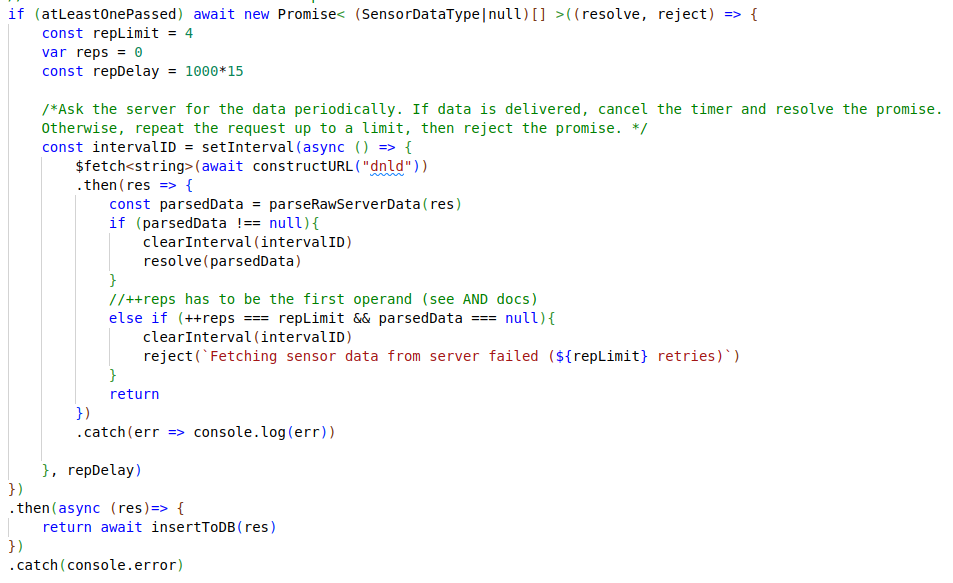
\includegraphics[width=\textwidth]{zdj/app/poll-fragment.png}
    \caption{Fragment funkcji odpowiedzialnej za wysyłanie do serwera IQRF Cloud odpytań o stan czujników}
    \label{iqrf-query1}
\end{figure}

Adres zapytania jest konstruowany za pomocą funkcji widocznej na Rys. \ref{construct-url}

\begin{figure}[H]
    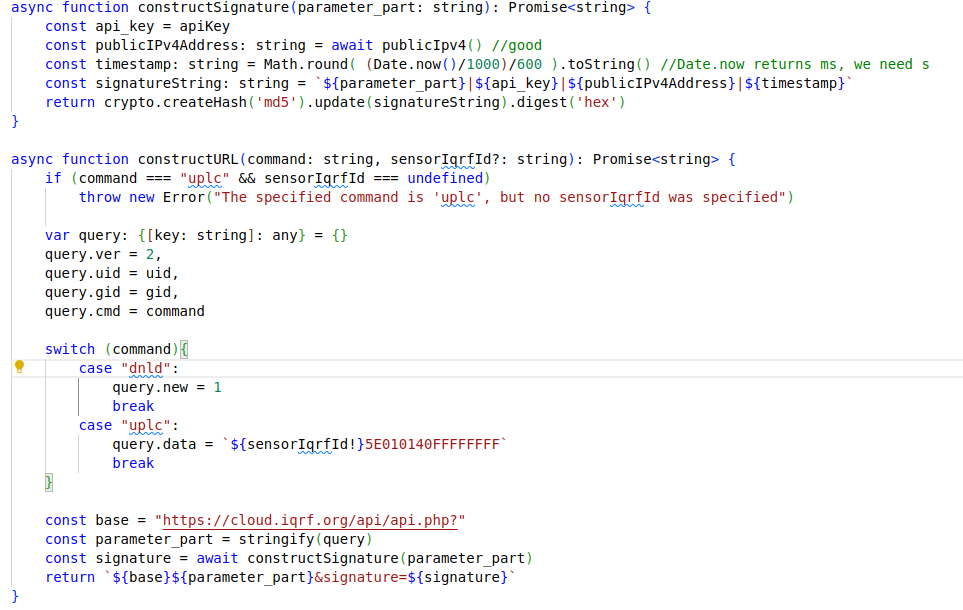
\includegraphics[width=\textwidth]{zdj/app/construct-url.png}
    \caption{Funkcje konstruujące adres zapytania}
    \label{construct-url}
\end{figure}

Ilość takich zapytań jest równa ilości czujników istniejących
w bazie danych. Parametry zapytania 'ver', 'gid' oraz 'uid' to odpowiednio wersja API serwera, ID bramki IQRF oraz ID użytkownika i dla każdego zapytania są one 
stałe. Parametr 'cmd' dla tego zapytania przyjmuje wartość 'uplc' - upload command, co powoduje przesłanie do serwera IQRF Cloud danych z parametru 'data'.
W przypadku tego zapytania do IQRF Cloud przesyłane są dane specyfikujące z jakiego czujnika mają zostać pobrane dane, oraz jakie dane to mają być. 
Przykładowo: \textbf{01005E010140FFFFFFFF} oznacza pobór danych o temperaturze, wilgotności i dwutlenku węgla z czujnika o ID 1. Więcej informacji na ten temat 
można odczytać z rodziału '\nameref{system}' oraz z dokumentacji \cite{protronix-comms}.

Dane z czujników są zapisywane na serwerze IQRF Cloud, nie na serwerze tej aplikacji webowej, trzeba je więc pobrać w osobnym zapytaniu. 
Po wysłaniu pierwszego zapytania (cmd=uplc) serwer oczekuje gotowej odpowiedzi do odczytania z serwera IQRF Cloud. Jako, że tylko serwer tej aplikacji może inicjować przesył danych
konieczne było zastosowanie mechanizmu pollingu, w którym serwer co jakiś czas wysyła zapytanie do IQRF Cloud o to, czy odpowiednie dane są gotowe do odbioru

Zapytanie, jakie serwer aplikacji wysyła do serwisu IQRF Cloud jest tym razem \\
'https://cloud.iqrf.org/api/api.php?ver=2\&gid=xxx\&uid=xxx\\\&cmd=dnld\&new=1\&signature=xxx'. \\ W porównaniu z poprzednim zapytaniem zmienia się tutaj wartość parametru
'cmd' na 'dnld' - download, oraz zostaje dodany nowy parametr, 'new=1', który pozwala na pobieranie najnowszych danych z serwera. Jeżeli serwe IQRF Cloud dostarczy dane
w odpowiednim czasie i odpowiedniej liczbie prób, serwer przechodzi do następnej fazy, czyli filtrowania i formatowania danych. W przypadku braku odpowiedzi po
pewnej liczbie zapytań serwer przestaje odpytywać zewnętrzny serwer i po odczekaniu pozostałego w tym cyklu czasu przechodzi do następnego cyklu.

\subsection{Filtrowanie i formatowanie danych}
Dane pobrane z serwera IQRF Cloud mają postać niezdatną do zapisu w bazie danych oraz nieprzyjazną dla użytkownika końcowego. Dodatkowo, nie wszystkie dane pobrane z 
serwera zawierają informacje o stanie czujników - niektóre ramki są informacją, że dany czujnik odebrał zapytanie, dany czujnik istnieje w systemie lub o podłączeniu
bramki do sieci. Z punktu widzenia aplikacji nie są to istotne dane.

Dane pobrane z serwera mają format przedstawiony na Rys. \ref{data-format}

\begin{figure}[H]
    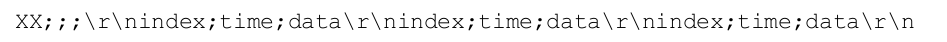
\includegraphics[width=\textwidth]{zdj/app/data-shape-iqrf.png}
    \caption{Format danych odbieranych z IQRF Cloud \cite{iqrfcloud-guide}}
    \label{data-format}
\end{figure}

Taki surowy ciąg danych (maksymalnie do 1000 rekordów jednocześnie) jest przekazywany do funkcji widocznej na Rys. \ref{data-formatter}, która z powyższego ciągu znaków
wydziela pojedyncze rekordy.

\begin{figure}[H]
    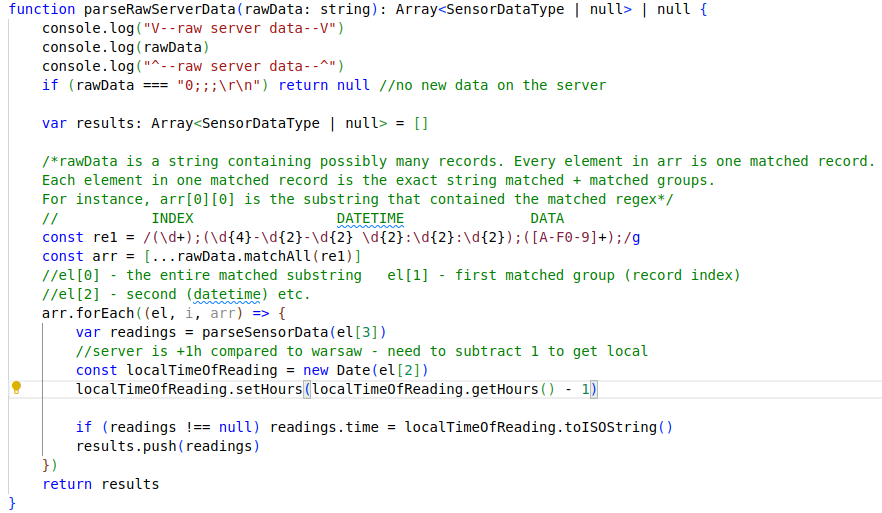
\includegraphics[width=\textwidth]{zdj/app/parse-raw.png}
    \caption{Funkcja formatująca surowe dane}
    \label{data-formatter}
\end{figure}

Każdy rekord jest pobierany iteracyjnie z tablicy wydzielonych rekordów do funkcji \\ \underline{parseSensorData}, gdzie zanim dojdzie do sformatowania rekordu 
dochodzi do jego filtracji w funkcji ukazanej na Rys. \ref{data-filter} - sprawdzenia, czy rekord zawiera potrzebne dane oraz czy pochodzi z czujnika zarejestrowanego w systemie. Rekordy, które nie przeszły filtracji 
są zwracane jako wartość \textbf{null}

\begin{figure}[H]
    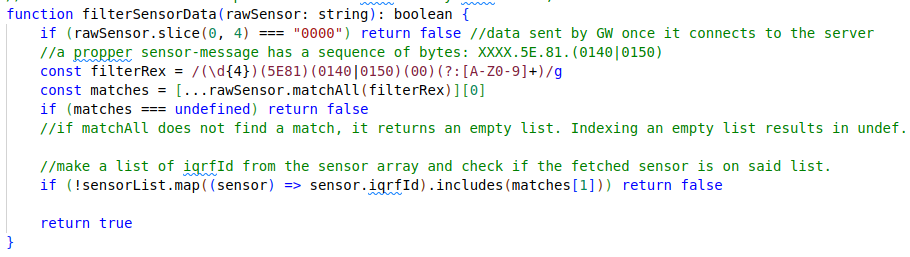
\includegraphics[width=\textwidth]{zdj/app/filter.png}
    \caption{Funkcja filtrująca dane niezawierające użytecznych danych}
    \label{data-filter}
\end{figure}

Następnie każdy rekord jest parsowany i zapisywany do obiektu typu SensorDataType (Rys. \ref{data-type}). Data pobranego rekordu opiera się na formacie ISO 8601 (YYYY-MM-DDTHH:mm:ss.sssZ). 
Parsowanie rekordu polega na przepuszczeniu go przez szereg wyrażeń regularnych (RegEx'ów), a tak powstałe tokeny są następnie zamieniane na liczby
dziesiętne i mnożone przez odpowiednie stałe \cite{protronix-comms} w celu otrzymania wyniku w rzeczywistych jednostkach za pomocą funkcji ukazanej
na Rys. \ref{record-after-parsing}.

\begin{figure}[H]
    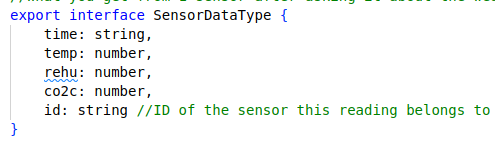
\includegraphics[width=\textwidth]{zdj/app/type.png}
    \caption{Typ danych jakie powstają w wyniku parsowania}
    \label{data-type}
\end{figure}

\begin{figure}[H]
    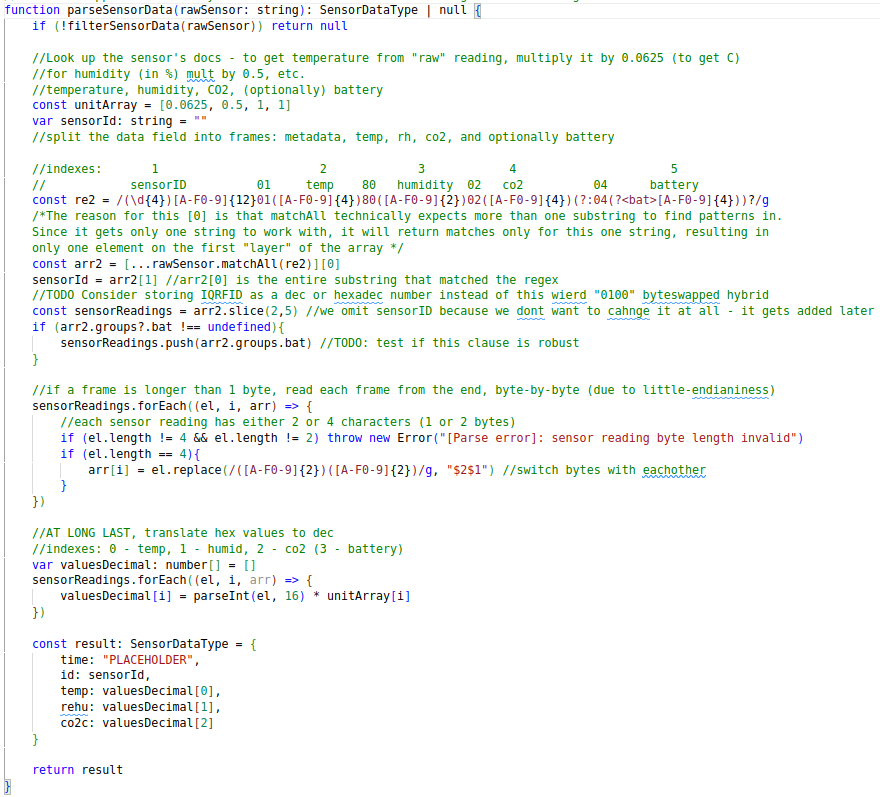
\includegraphics[width=\textwidth]{zdj/app/parse-sensor.png}
    \caption{Funkcja parsująca pojedynczy rekord do postaci liczbowej}
    \label{record-after-parsing}
\end{figure}

\subsection{Zapis do bazy danych}

Po zakończonym procesie filtrowania i formatowania dane są zapisywane do bazy danych. Zapis do bazy jest konieczny, gdyż serwer IQRF Cloud może przechowywać
jednocześnie tylko 2000 rekordów, w co wliczają się rekordy nie niosące żadnej informacji o czujnikach.

\subsection{Baza danych}

Jak wcześniej wspomniano, za silnik wybrano nierelacyjną bazę danych MongoDB. W tej bazie istnieją tylko dwie kolekcje - jedna z nich zawiera wszystkie zarejestrowane 
czujniki, druga zaś wszystkie odczyty ze wspomnianych czujników. Przykładowe rekordy zostały ukazane na Rys. \ref{db-records}

\begin{figure}[H]
\begin{subfigure}{0.5\textwidth}
    \centering
    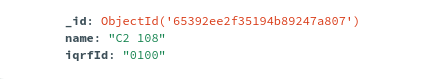
\includegraphics[width=\linewidth]{zdj/app/db-sensor.png}
    \caption{Wygląd pojedynczego rekordu z kolekcji\\ 'Sensors' przedstawiającego czujnik w bazie danych}
\end{subfigure}
\hspace{1cm}
\begin{subfigure}{0.5\textwidth}
    \centering
    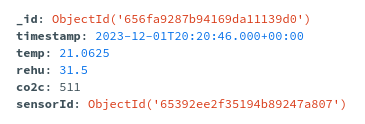
\includegraphics[width=0.8\linewidth]{zdj/app/db-reading.png}
    \caption{Wygląd pojedynczego rekordu z kolekcji\\ 'Records' przedstawiającego odczyt z czujnika w bazie danych}
\end{subfigure}
   
\caption{Struktura rekordów w bazie danych}
\label{db-records}
\end{figure}


